\section{Fine-tuning}

As a warmup, we will perform perhaps the most straightforward form of $k$-shot learning with a pre-trained model: directly fine-tuning the entire model on the $k$ examples. We will use two different sizes of smaller BERT models that have been compressed through distillation.\footnote{See \href{https://arxiv.org/pdf/1908.08962.pdf}{here} to learn more about this class of distilled BERT models. For final projects involving language models, these smaller BERT models may be useful for performing compute-friendly experiments!}

\begin{enumerate}[label={1.\alph*}]
    \item \points{3a} {\bf Implement Parameter-efficient Fine Tine}

Finish the implementation for each version of parameter-efficient fine-tuning for GPT-2-Medium in 

\texttt{ft.py:parameters\_to\_fine\_tune()}:

\begin{enumerate}[label=(\roman*)]
    \item \texttt{last}: Fine-tune only the last 2 transformer blocks
    \item \texttt{first}: Fine-tune only first 2 transformer blocks
    \item \texttt{middle}: Fine-tune only middle 2 transformer blocks
\end{enumerate}
This step simply requires selecting the correct subset of parameters for each version listed above in 

\texttt{parameters\_to\_fine\_tune()}. Keep in mind you should be returning an iterable of \texttt{nn.Parameter} here, not \texttt{nn.Module}.
    \item {\bf Observe Fine-Tuning}

\begin{enumerate}[label=(\roman*)]
    \item \points{1bi} {\bf Run Fine-Tuning}

Run the command:
    
{\small\texttt{python3 main.py --task run\_ft --model bert-tiny,bert-med --dataset amazon --k 1,8,128}}

to fine-tune two sizes of BERT models on the Amazon Reviews dataset for various values of $k$. While debugging, you can pass only one value for each of the arguments to run only that subset, e.g. \texttt{python3 main.py --task run\_ft --model bert-tiny --dataset amazon --k 1}.

If you see a log message like \texttt{Some weights of the model checkpoint...}, this is expected, since the pre-trained model does not contain a prediction head for our task (this is why we need to fine-tune!).

To plot your results, run the command:

{\small\texttt{python3 main.py --task plot\_ft --model bert-tiny,bert-med --dataset amazon --k 1,8,128}}

Your plot should look as follows:
\begin{center}
    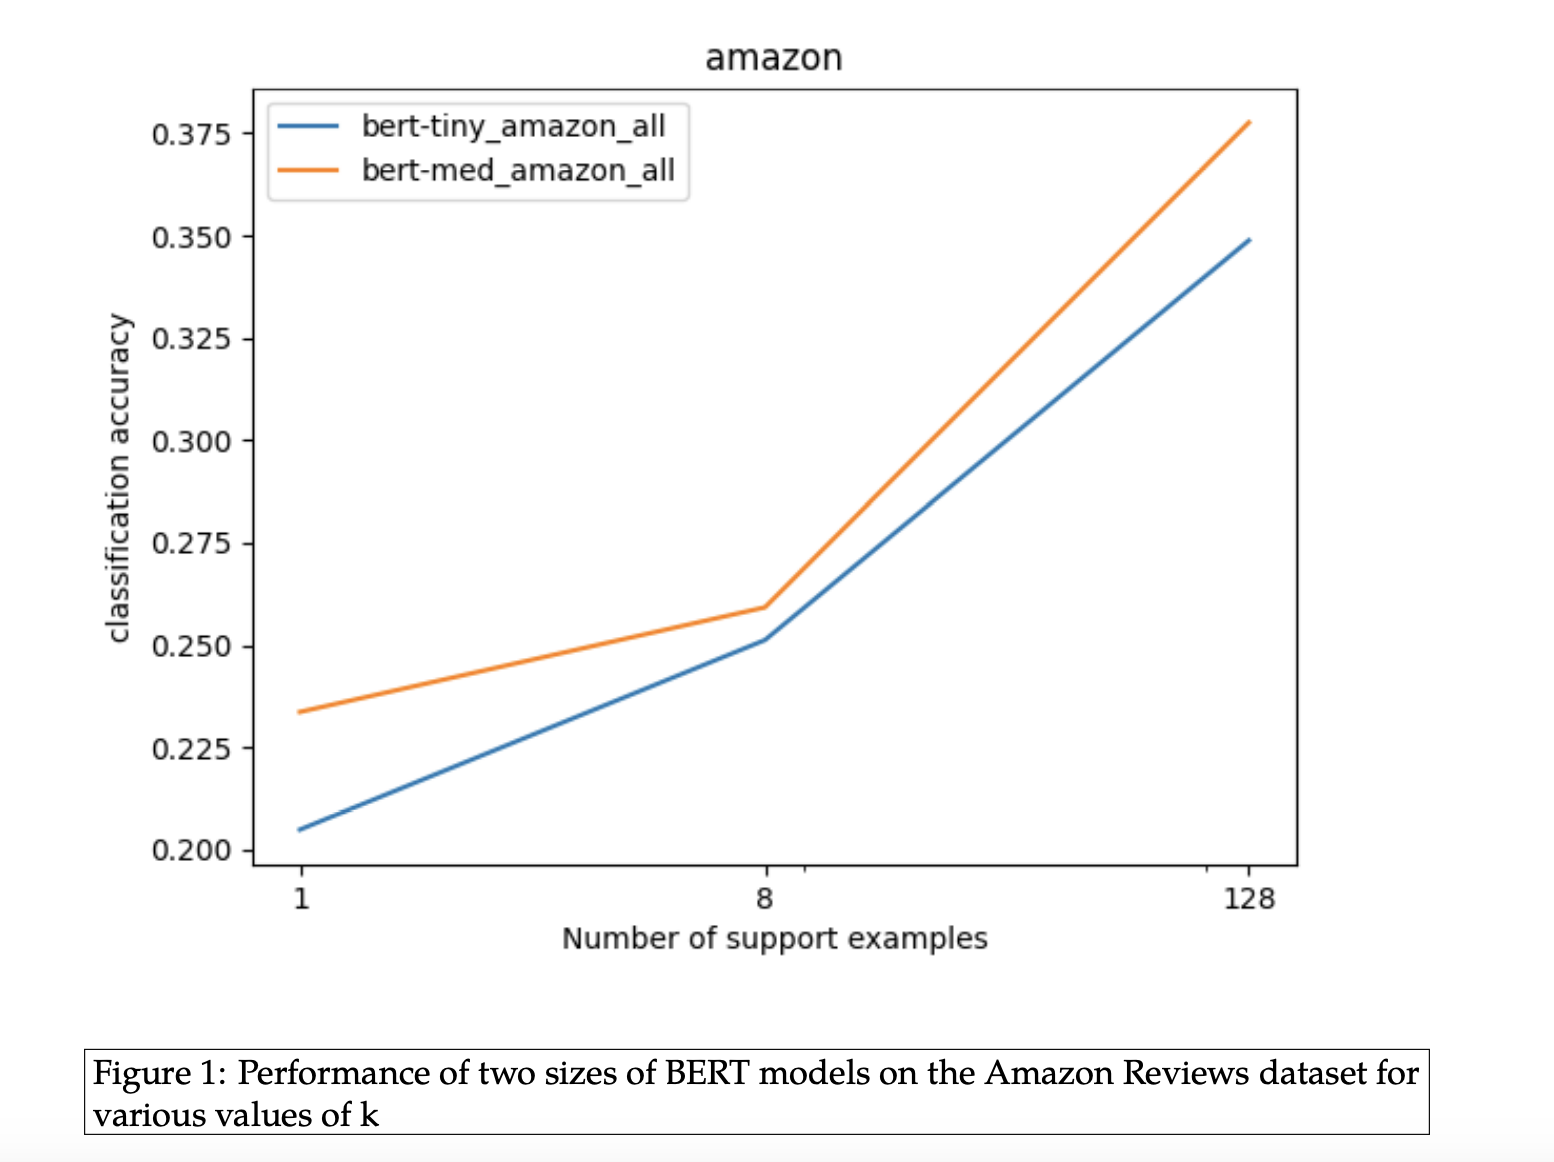
\includegraphics[width=0.75\linewidth]{./figures/finetune-1b}
\end{center}

\clearpage

    \item \points{1bii} {\bf Reason on Fine-Tuning}

In one sentence, what do you notice about the performance of the two model scales?

\clearpage

\end{enumerate}

\clearpage

    \item \points{1c} {\bf Storage for Fine-Tune}

If we fine-tune the all of our model parameters for each task, we must save a new complete copy of the model's parameters for each new task. As an example, a BERT-mini model similar to the ones you just fine-tuned has approximately 11.2 million parameters; assuming parameters are represented as 4-byte floats, after fine-tuning on a new task, how much disk space do we need to store the new fine-tuned model parameters?
    \item \points{1d} {\bf Disk Space}

Google's recent large language model \href{https://storage.googleapis.com/pathways-language-model/PaLM-paper.pdf}{PaLM} has 540 billion parameters. How much disk space would be needed to store a new fine-tuned version of this model, assuming parameters are represented as 4-byte floats?
\end{enumerate}